Wie in den Kapiteln \ref{chp:explizite_interaktion} und \ref{chp:implizite_navigation} erläutert wird, können verschiedene implizite und explizite Techniken verwendet werden um alle Freiheitsgrade der Navigationsmanipulation in einer virtuellen Szene zu steuern. Durch die Vielzahl der unterschiedlichen Modi für die Interaktion, ist es wichtig geeignete Kriterien zu definieren, nach denen zwischen den Techniken gewechselt werden kann. 
\\\\
In Abschnitt \ref{sec:evaluierung_der_bildschirmkontakte} wird eine Herangehensweise an diese Problematik vorgestellt, die anhand der Evaluierung von Kontaktpunkten auf dem Bildschirmtisch eine geeignete Interaktionsform ableitet. Abschnitt \ref{sec:menu_elemente} zeigt wie Menüstrukturen zur Festlegung des Navigationsmodus beitragen können. Zuletzt werden in Abschnitt \ref{sec:diskussion_wechsel} beide Ansätze verglichen und auf ihre Vorteile und Limitierungen untersucht.


\section{Evaluierung der Bildschirmkontakte}
\label{sec:evaluierung_der_bildschirmkontakte}

Die in Kapitel \ref{chp:mser} beschriebene, zugrunde liegende Touch-Eingabeerkennung gibt Aufschluss über vom Nutzer platzierte Bildschirmkontaktpunkte. Des Weiteren ermöglicht sie die Zuordnung dieser Fingerpositionen zu einzelnen Händen. Obwohl hierbei eine genaue Hand-Nutzer Zuweisung nicht möglich ist, kann die Evaluierung der gegebenen Eingabeinformationen bereits effektiv als Kriterium zur Festlegung des Navigationszustands genutzt werden.
\\\\
In kollaborativen Anwendungsszenarien ist gemeinsame Analyse der gebotenen virtuellen Inhalte stark an das Zeigen auf bestimmte Bereiche der Visualisierung gebunden. Wie in der Anforderungsanalyse (siehe Kapitel \ref{chp:wahrnehmungskonflikte_und_loesungsansaetze}) vorgestellt, verlieren Nutzer durch Stereoparallaxe leicht die visuelle Wahrnehmung des physischen Bildschirms. In Folge dessen kann es passieren das Nutzer versehentlich mit einem Finger die Bildschirmoberfläche berühren und damit ungewollt Manipulationen an der Applikation vornehmen. Um diesen Eingabekonflikt zu verhindern, wird die Eingabe einer Hand nur für die Interaktion angewendet, wenn der Anwender mehr als einen Finger auf die Bildschirmoberfläche legt. 
\\\\
Da für die Berechnung der Manipulationsparameter nur ein Punkt der jeweiligen Hand als Eingabe nötig ist, wird eine Handzentrumsposition ermittelt. Diese wird aus den Positionen aller enthaltenen Finger berechnet. Sie kann wahlweise durch den gemittelten Positionswert aller Kontaktpunkte, oder den Mittelpunkt des fingerumschließenden Rechtecks definiert sein. Für die Berechnung der Manipulationsparameter wird die relative Translation der gesamten Hand des Nutzers über den Bildschirm auf die jeweiligen Interaktionsmodi übertragen. Hierbei ist zu beachten, dass das die berechnete Handzentrumsposition kein fester Punkt auf der Hand des Nutzers ist. Folglich führt das Aufsetzen oder Entfernen von Fingern an der interagierenden Hand ebenfalls zur Verschiebung des Handzentrums. Die Auswirkung dieser Translation auf die Manipulation sollte verhindert werden, da sie zu sprunghaften Veränderungen der Applikation führt.

\begin{figure}
	\begin{center}
		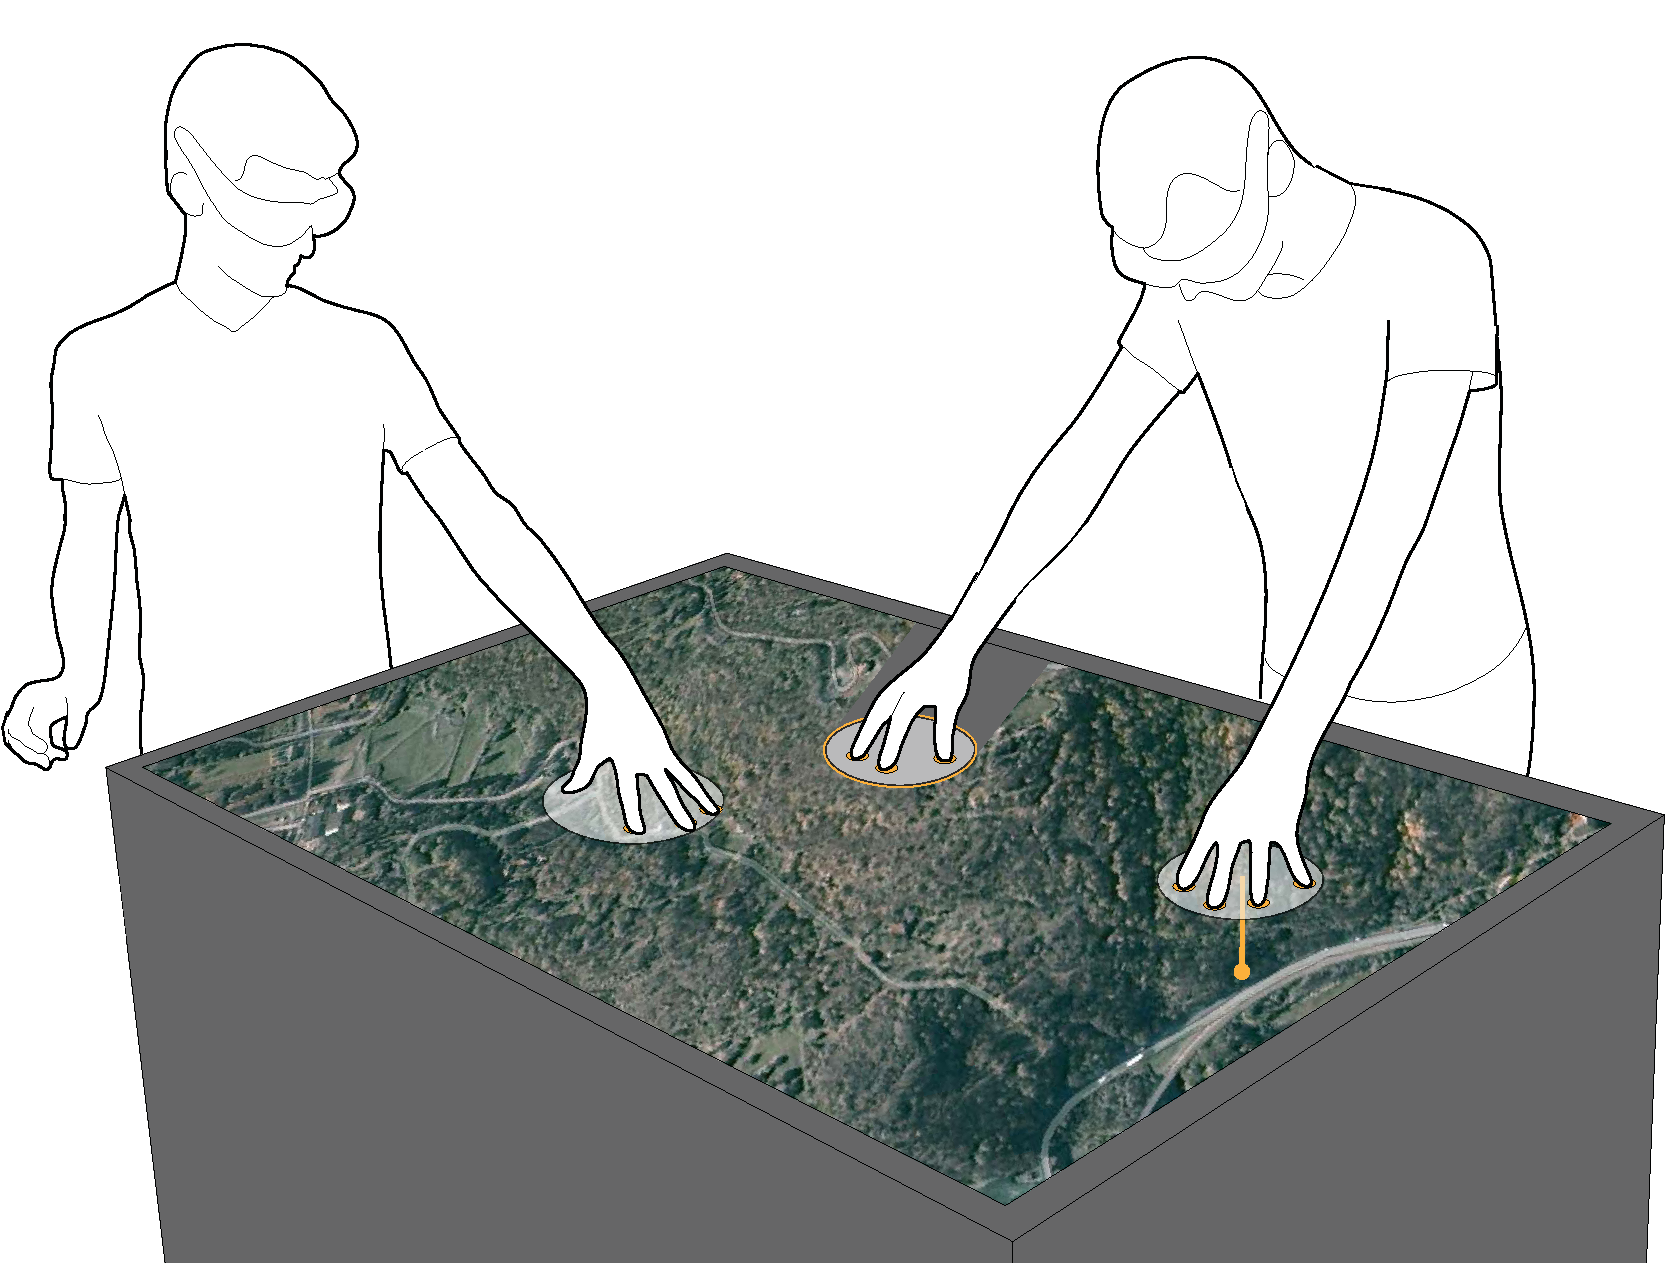
\includegraphics[width=12cm]{img/drei_kontakte.pdf}
	\end{center}
	\caption{Zwei Nutzer interagieren gleichzeitig mit der Bildschirmfläche. Dies kann Konflikte bei der Eingabe hervorrufen. Aus diesem Grund werden nur maximal zwei Kontakte zur Manipulation der Applikation zugelassen. Alle bei Überschreitung dieser Limitierung gelieferten Eingaben werden vom System ignoriert.}
	\label{fig:drei_kontakte}
\end{figure}

Vergleicht man alle in den Kapiteln \ref{chp:explizite_interaktion} und \ref{chp:implizite_navigation} vorgestellten Interaktionsmodi hinsichtlich ihrer zur Berechnung der Manipulation verwendeten Kontaktpunkte wird deutlich, dass keine der Techniken mehr als zwei aktuelle Inputpositionen nutzt. Eingabekonflikte entstehen häufig, wenn mehrere Anwender gleichzeitig mit dem Bildschirmtisch zu interagieren versuchen. Dieses Problem kann dadurch begrenzt werden, dass nicht mehr als zwei Hände zur Interaktion zugelassen werden. Demzufolge werden genau die beiden Hände zur Eingabe genutzt, welche den Projektionstisch früher berühren. Abbildung \ref{fig:drei_kontakte} illustriert die Auswirkung dieser Technik auf ein beispielhaftes Szenario.
\\\\
Die beschriebenen Navigationstechniken lassen sich ebenfalls durch Auswertung der vom Nutzer aufgesetzten Kontaktpunkte auswählen. Nach der oben genannten Erklärung wird für die Eingabe eines einzelnen Fingers kein Navigationsmodus betreten.
\\\\
2D Translation ist einhändig bedienbar. Gleiches gilt für die in Abschnitt \ref{sec:3d_rotation} beschriebene 3D Rotation, falls die interagierende Hand mehr als einen Finger beinhaltet. Diese Technik wäre auch mit den Zentrumspositionen zweier Hände berechenbar. Zugunsten der Verständlichkeit der Interaktion und um eine klare Definition für die Wahl des Modus zu gewährleisten, wird der 3D Rotationsmodus jedoch ausschließlich bei der Eingabe mit zwei Fingern, bei genau einer aufgelegten Hand gesteuert. Somit bleiben Dreifinger-, Vierfinger- und Fünffinger-Einhand-Interaktion für die Kontrolle der 2D Translation.
\\\\
Für den RTS+L Modus (siehe Abschnitt \ref{sec:definition_levelling}) werden zur Berechnung aller Manipulationsparameter zwei Kontaktpunkte benötigt. Selbiges gilt für die in Abschnitt \ref{sec:3d_translation} vorgestellte 3D Translation. Da letztere Interaktionstechnik jedoch keine Auswirkungen auf Skalierung und Rotation hat, wird ein allgemeiner Translationsmodus definiert. Dieser schließt die Verwendung von einhändiger 2D Translation ein. Setzt ein Nutzer nach einem bestimmten Zeitintervall der Einhand-Interaktion eine zweite Hand auf, wird die  3D-Translation angewandt. Demzufolge wird RTS+L bedient wenn zwei Hände mit zeitlicher Differenz kleiner des bestimmten Zeitintervalls aufgesetzt werden. Ein Zustandsdiagramm (siehe Abbildung XX) verdeutlicht den Umgang mit den Navigationsmodi durch Evaluierung der Bildschirmkontakte.


\section{Auswahl durch Menüelemente}
\label{sec:menu_elemente}

Die Nutzung von Betriebssystemen und sonstigen Programmen mit Grafischer Benutzeroberfläche macht den Umgang mit Menüstrukturen zur Konfiguration von Arbeitsabläufen alltäglich. Aus diesem Grund sind schaltbare, geometrische Flächen in Null-Parallaxe eine naheliegende Lösung zur Filterung von Navigationsmodi. Nach diesem Ansatz wird jeder Interaktionstechnik eine in der Bildebene liegende Geometrie zugeordnet. Selektiert der Nutzer eine dieser und ist der referenzierte Modus aktiv, so wird dieser deaktiviert. Ist er deaktiviert, so erfolgt eine Aktivierung. Sind mehrere Modi gleichzeitig eingeschaltet, wird die Wahl der Technik nach den in Abschnitt \ref{sec:evaluierung_der_bildschirmkontakte} ermittelt.   
\\\\
Herrlich et al. stellen mit ihrer Technik \emph{PieRotate} einen Ansatz zur Separierung der Freiheitsgrade der dreidimensionalen Rotation mit Touch-Eingaben vor \cite{herrlich:2011}. \emph{PieRotate} teilt den Interaktionsraum zur Manipulation eines Objekts in drei Zonen auf. Durch eine Rotationsgeste in der jeweiligen Zone, kann das Objekt um die zugewiesene Achse gedreht werden. Diese Lösung lässt sich auf die Umschaltung verschiedener Navigationsmodi übertragen. Demnach werden Interaktionsterritorien definiert, in denen bestimmte Techniken verwendet werden, welche durch den Nutzer erzeugbar und konfigurierbar sind. Bier et al. beschreiben die Verwendung von \emph{Magic Lenses} zur Erzeugung von Filtereffekten in bestimmten Arealen des Bildes. 
\emph{Magic Lenses} sind nach dieser Entwicklung durchsichtige, fensterartige Interfaces, welche das Rendering der unter ihnen liegenden Applikationsinhalte beeinflussen.\newpage Ein Anfasser in der Ecke der \emph{Magic Lense} macht das Werkzeug durch Dragging beweglich.

\begin{figure}
	\begin{center}
		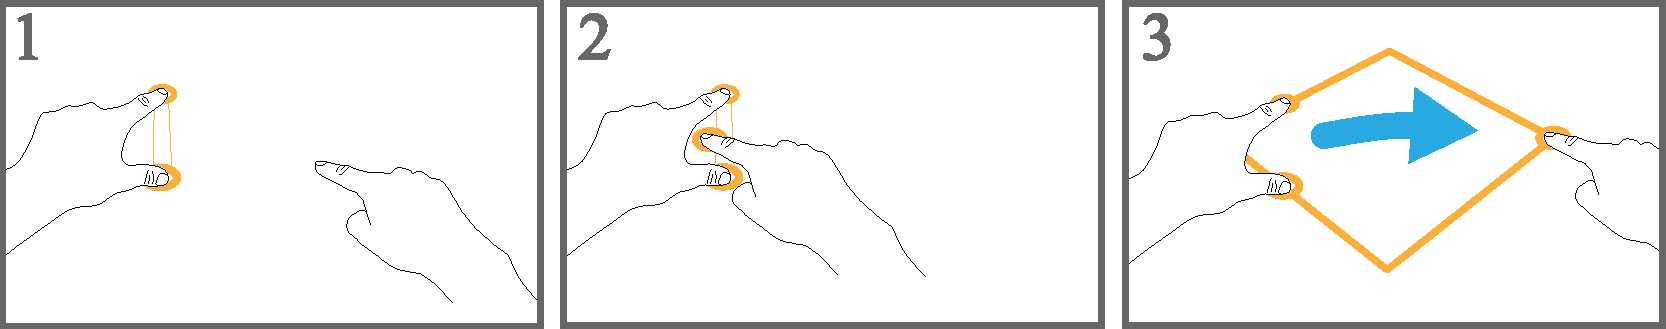
\includegraphics[width=12cm]{img/menu_geste.pdf}
	\end{center}
	\caption{Die Erzeugung von Menuelementen durch eine Touch gesteuerte Crossing Geste nach Accot und Zhai \cite{accot:2002}. In Bild 1 ist die visuelle Verbindungslinie zwischen zweie Fingern zu sehen. Darstellung 2 zeigt die Bestrebung des Anwenders diese zu durchkreuzen um ein neues Fenster zu erstellen. Zuletzt kann dieses durch fortwährende Streichbewegung skaliert werden, wie Abbildung 3 zeigt.}
	\label{fig:menu_geste}
\end{figure}

Die Erzeugung von Menüelementen und Fenstern lässt sich durch die Einführung einer zugewiesene Touch-Geste ergänzen. Demnach führt das Aufsetzen zweier Finger einer Hand, zur Konstruktion einer visuellen Verbindungslinie zwischen den Fingern. Inspiriert vom \emph{Crossing}-Verfahren nach Accot und Zhai \cite{accot:2002}, führt das Durchstreichen dieser Linie zum Öffnen eines Fensters. Dieses dehnt sich durch die fortwährende Bewegung des durchstreichenden Fingers aus, bis er die Eingabefläche verlässt. Eine Implementierung dieses Konzepts ist im Zuge der Arbeit nicht entstanden. In Abbildung \ref{fig:menu_geste} wird dieses Konzept visualisiert.


\section{Diskussion}
\label{sec:diskussion_wechsel}

\begin{figure}
	\begin{center}
		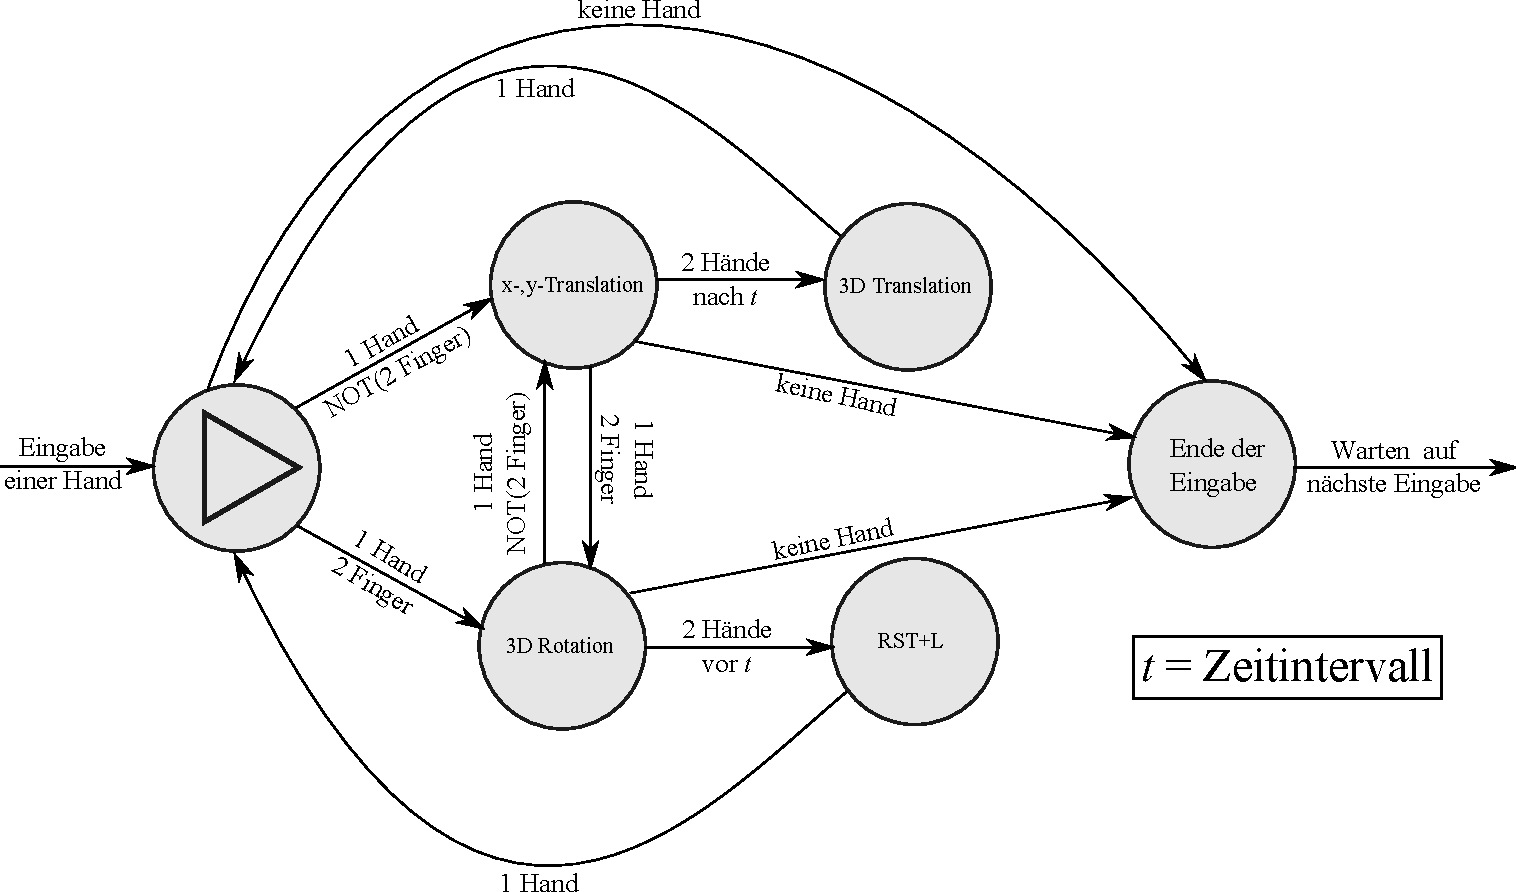
\includegraphics[width=12cm]{img/zustandsdiagramm.pdf}
	\end{center}
	\caption{Ein Zustandsdiegramm welches die Übergänge zwischen den Interaktionsmodi visualisiert.}
	\label{fig:zustandsdiagramm}
\end{figure}

Die Evaluierung der Bildschirmkontakte nach Abschnitt \ref{sec:evaluierung_der_bildschirmkontakte} gibt dem Anwender die Möglichkeit allein durch verschiedene Bewegungsabfolgen zwischen einer Reihe von Navigationsmodi zu wechseln. Aufgrund dessen sind flüssige Interaktionsabläufe möglich. Der Nutzer muss sich hierzu jedoch eine Reihe von Regeln zur Verwendung der jeweiligen Techniken merken, was die intuitive Bedienung des Systems strapaziert. Folgendes Szenario hebt die Komplexität und den kognitiven Aufwand bei der Zustandsunterscheidung hervor:
\\
RTS+L und 3D Translation sind an einen zweihändigen Input gebunden. Die Entscheidung zur Aktivierung einer dieser Modi wird lediglich durch zeitliche Auswertung getroffen. Bei der Analyse des in Abbildung \ref{fig:zustandsdiagramm} dargestellten Zustandsdiagramms wird deutlich, dass der RTS+L Modus durch kurzzeitiges Anheben einer Hand verlassen wird. Ab diesem Zeitpunkt wird durch erneutes Aufsetzen der 3D Translationsmodus aktiviert. RTS+L kann erst durch Entfernen der zweiten Hand vom Bildschirm und Aufsätzen beider Hände innerhalb des Zeitintervalls nochmals genutzt werden.
\\\\
Die Einbindung einer Menüstruktur nach Abschnitt \ref{sec:menu_elemente} gibt dem Nutzer durch visuelle Rückmeldung einen Überblick über alle verfügbaren Modi. Nach den Ansprüchen des jeweiligen Nutzers kann so individuell die Zustandsunterscheidung erleichtert werden. Eine Verwendung aller Navigationsmodi nach Abschnitt \ref{sec:evaluierung_der_bildschirmkontakte} ist noch immer möglich. Durch Visualisierung von Menüstrukturen auf der Bildebene werden hingegen Teile der Applikation verdeckt. Außerdem schmälert der durch Menüelemente eingenommene Raum die Interaktionsfläche für die Navigationsmanipulation. Zusätzlich verdecken Modellinhalte in Negativ-Parallaxe möglicherweise die dargestellten funktionalen Bestandteile der Benutzeroberfläche, was den Umgang mit ihnen erschwert. 
\\\\
Keiner der in diesem Kapitel genannten Ansätze vermeidet das Auftreten von Eingabekonflikte zwischen den Nutzern vollständig. Durch die fehlende Hand-Nutzer Zuordnung kann bei der zweihändigen Interaktion nicht verhindert werden, dass zwei Nutzer mit je einer Hand Veränderungen am Applikationszustand vornehmen.
